\chapter{Phương pháp đề xuất}
\label{Chapter3}

\section{Ý tưởng ban đầu} 

Dựa trên các nghiên cứu liên quan, nhóm đề xuất xây dựng một hệ thống học sâu đa phương thức nhằm khai thác đồng thời thông tin từ ảnh X-quang và dữ liệu lâm sàng văn bản. Đặc biệt, hệ thống được thiết kế theo hướng tích hợp tri thức y khoa nhằm nâng cao khả năng học ít mẫu và phát hiện dữ liệu ngoài phân phối. Cụ thể, kiến trúc bao gồm các thành phần chính như sau:
    \begin{itemize}
        \item \textbf{Tiền xử lý văn bản với UMLS}: Phương pháp sử dụng GLiNER để trích xuất các tình trạng y khoa cùng với mức độ và vị trí từ báo cáo chẩn đoán ảnh X-quang, sau đó ánh xạ chúng vào hệ thống phân loại UMLS (Unified Medical Language System) để chuẩn hóa và liên kết tri thức từ đó xây dựng được các câu mô tả nhằm làm giàu ngữ nghĩa.
        \item \textbf{Bộ mã hóa ảnh:} Kế thừa lại mô hình ViT-Base của phương pháp BiomedCLIP \cite{BiomedCLIP}
        \item \textbf{Bộ mã hóa văn bản:} Kế thừa lại mô hình PubMedBERT của phương pháp BiomedCLIP \cite{BiomedCLIP}
        \item \textbf{Bộ dung hợp dữ liệu:} Kỹ thuật Bidirectional Cross-Attention được xây dựng dựa trên cơ chế cross-attention 
        nhằm học mối quan hệ ngữ nghĩa giữa đặc trưng hình ảnh và đặc trưng văn bản y khoa.
        \item \textbf{Bộ phân loại:} Dùng phương pháp metric-based few-shot learning với một prototypical network, nhãn được quyết định bởi khoảng cách
         đến các prototype trong không gian biểu diễn chung, 
        thay vì lớp phân loại truyền thống làm ràng buộc mô hình phân loại vào các nhãn đã biết, 
        giúp phát hiện dữ liệu ngoài phân phối khi khoảng cách đó vượt quá ngưỡng xác định.

    \end{itemize}
    Đồng thời, các trọng số attention và thông tin từ tri thức y khoa được khai thác để trực quan hóa và giải thích kết quả dự đoán.

\section{Tiền xử lý văn bản với UMLS}
\begin{figure}[H]
    \centering
    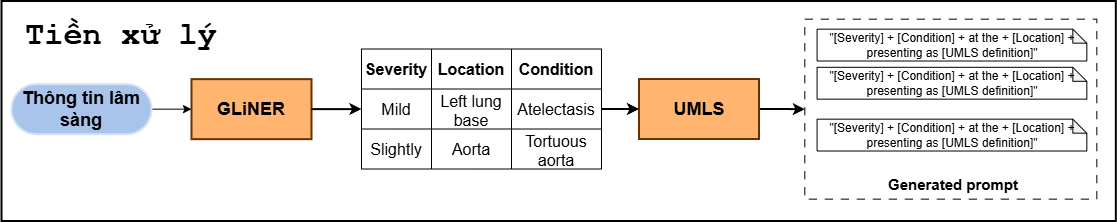
\includegraphics[width=1\linewidth]{images/preprocessing.png}
    \caption{Công đoạn Tiền xử lý văn bản với UMLS.}
    \label{fig:preprocessing}
\end{figure}
Công đoạn tiền xử lí được thực hiện ở toàn bộ 2 giai đoạn offline và online của phương pháp, 
sử dụng GLiNER để trích xuất các tình trạng y khoa cùng với mức độ và vị trí từ báo cáo chẩn đoán ảnh X-quang, 
sau đó ánh xạ chúng vào hệ thống phân loại UMLS (Unified Medical Language System) để chuẩn hóa 
và liên kết tri thức từ đó xây dựng được các câu mô tả nhằm làm giàu ngữ nghĩa.


\section{Giai đoạn off-line}
Giai đoạn off-line nhằm xây dựng bộ tham số cho mô hình, thiết lập không gian biểu diễn chung và học cách dung hợp giữa đặc trưng hình ảnh X-quang và ngữ nghĩa y khoa.

Giai đoạn off-line gồm 2 công đoạn: Domain-Adaption và Fine-tuning. 
Trong đó, công đoạn Domain-Adaption nhằm mục đích giúp mô hình thích nghi từ miền dữ liệu tiền huấn luyện lớn sang miền dữ liệu y khoa đích của bài toán, 
trong khi công đoạn Fine-tuning tập trung vào việc tối ưu hóa khả năng dung hợp dữ liệu 
và phân loại trên tập dữ liệu mục tiêu.

\subsection{Domain-Adaption với kỹ thuật LoRA}
\begin{figure}[H]
    \centering
    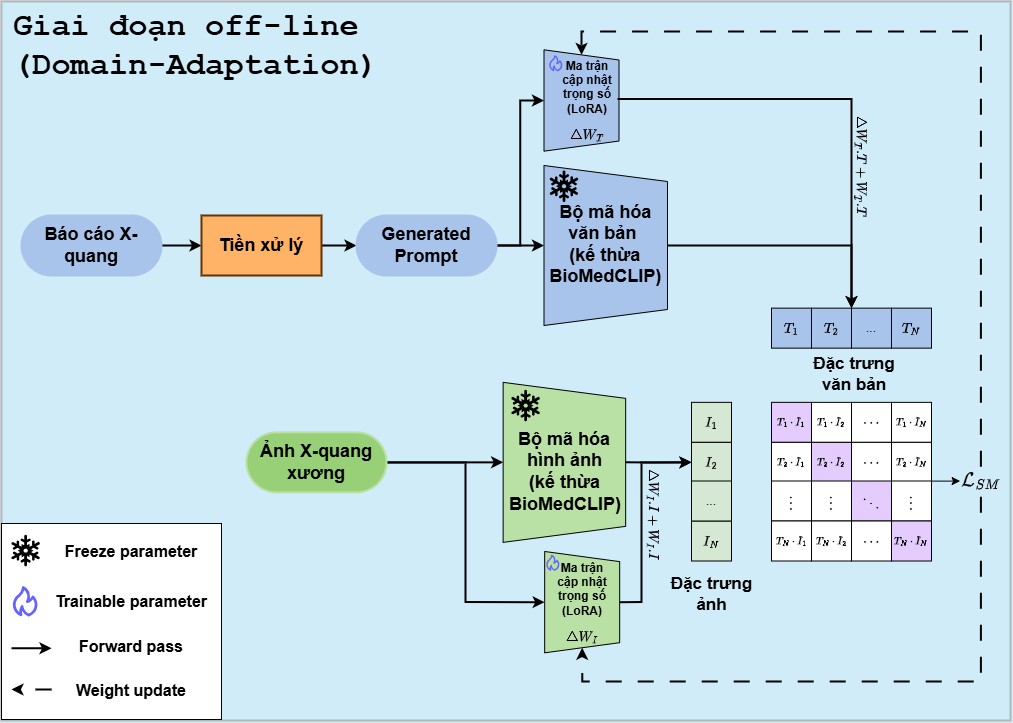
\includegraphics[width=1\linewidth]{images/domain-adaption.png}
    \caption{Sơ đồ chung của hệ thống trong công đoạn Domain-Adaption.}
    \label{fig:domain-adaption}
\end{figure}

Trong công đoạn này, mục tiêu chính giúp mô hình học cách biểu diễn sao cho các cặp ảnh và báo cáo khám tổng quát chung lớp nằm gần nhau hơn trong không gian biểu diễn bằng cách tối ưu hàm mất mát khớp ngữ nghĩa (Semantic Matching Loss), 
mô hình tuân theo framework contrastive learning để căn chỉnh bộ mã hóa BiomedCLIP về miền dữ liệu X-Quang xương được sử dụng, 
với đầu vào là các cặp ảnh X-quang và phân tích ảnh tương ứng của bác sĩ. Dữ liệu được đưa vào bộ mã hóa tương ứng để trích xuất đặc trưng, 
sau đó được chiếu vào không gian chung và chuẩn hóa để so sánh và thực hiện điều chỉnh. 
Kết quả là các cặp hình ảnh và văn bản giống nhau hoặc chung lớp nằm gần nhau hơn gọi là các semantic clusters, trong khi các cặp văn bản khác lớp sẽ nằm xa nhau hơn.

Nhóm thực hiện tinh chỉnh (fine-tuning) đồng thời Vision Encoder và Text Encoder bằng kỹ thuật LoRA (Low-Rank Adaptation): 
Thay vì tinh chỉnh toàn bộ trọng số của Vision Encoder và Text Encoder, kỹ thuật này đóng băng hai Encoder, sau đó chỉ tạo và cập nhật một ma trận nhỏ các tham số hạng thấp (low-rank) được chèn vào các khối Attention của các bộ mã hóa. Điều này giúp giảm thiểu rủi ro quá khớp (overfitting) và bảo tồn tri thức nền tảng của các mô hình mã hóa với trường hợp ít mẫu học.
    
    Để cập nhật trọng số của ma trận LoRA, nhóm sử dụng \textbf{Hàm mất mát Khớp ngữ nghĩa (Semantic Matching Loss - $\mathcal{L}_{SM}$)} nhằm đồng bộ hóa không gian biểu diễn đa phương thức. Thay vì tính toán trên các véc-tơ tổng, mô hình thiết lập ma trận tương đồng $s(I_i, T_j)$ dựa trên sự căn chỉnh giữa các vùng ảnh (patches) của ảnh $I_i$ và các từ vựng (tokens) của câu lệnh $T_j$. 

    Hàm mất mát được sử dụng là Semantic Matching Loss $\mathcal{L}_{SM}$ được định nghĩa là trung bình cộng của hai hàm mất mát tương phản hai chiều (Bi-directional Contrastive Loss), bao gồm chiều từ ảnh sang chữ ($\mathcal{L}_{I2T}$) và từ chữ sang ảnh ($\mathcal{L}_{T2I}$):
    \begin{equation}
        \mathcal{L}_{I2T} = -\frac{1}{N} \sum_{i=1}^{N} \log \frac{\exp(s(I_i, T_i) / \tau)}{\sum_{j=1}^{N} \exp(s(I_i, T_j) / \tau)}
    \end{equation}

    \begin{equation}
        \mathcal{L}_{T2I} = -\frac{1}{N} \sum_{i=1}^{N} \log \frac{\exp(s(I_i, T_i) / \tau)}{\sum_{j=1}^{N} \exp(s(I_j, T_i) / \tau)}
    \end{equation}

    \begin{equation}
        \mathcal{L}_{SM} = \frac{1}{2} (\mathcal{L}_{I2T} + \mathcal{L}_{T2I})
    \end{equation}
    trong đó, $N$ là kích thước mini-batch, $s(I_i, T_j)$ là điểm tương đồng ngữ nghĩa tổng hợp giữa ảnh $i$ 
    và văn bản $j$, và $\tau$ là siêu tham số nhiệt độ (temperature) giúp điều chỉnh độ nhạy của hàm phạt đối với 
    các mẫu âm tính (negative samples). Bằng cách tối ưu $\mathcal{L}_{SM}$, 
    mô hình đẩy các đặc trưng giải phẫu X-quang cục bộ hội tụ chặt chẽ về đúng định nghĩa y khoa của chúng 
    trong không gian chung.

Công đoạn Domain-Adaption giúp mô hình học cách biểu diễn sao cho các cặp ảnh và báo cáo khám tổng quát chung lớp nằm gần nhau hơn trong không gian biểu diễn, 
Semantic Matching Loss giúp các dữ liệu chung lớp nằm gần nhau thay vì ràng buộc như contrastive learning truyền thống rằng 
các cặp ảnh và báo cáo chung lớp dù không tương ứng dù nằm chung lớp vẫn phải nằm cách xa nhau ra. 
Điều này cực quan trọng với bài toán dữ liệu còn hạn chế, giúp tránh trường hợp dữ liệu nằm chung nhóm không hội tụ. 
Trong quá trình huấn luyện, đạo hàm từ hàm mất mát $\mathcal{L}_{SM}$ chỉ chảy qua và cập nhật ma trận 
$A \in \mathrm{R}^{r \times k}$ và $B \in \mathrm{R}^{d \times r}$ (với hạng $r \ll \min(d, k)$) của LoRA. 
Tổng số tham số cần học (learnable parameters) chiếm dưới 5\% toàn mạng.


\subsection{Fusion-learning}
\begin{figure}[H]
    \centering
    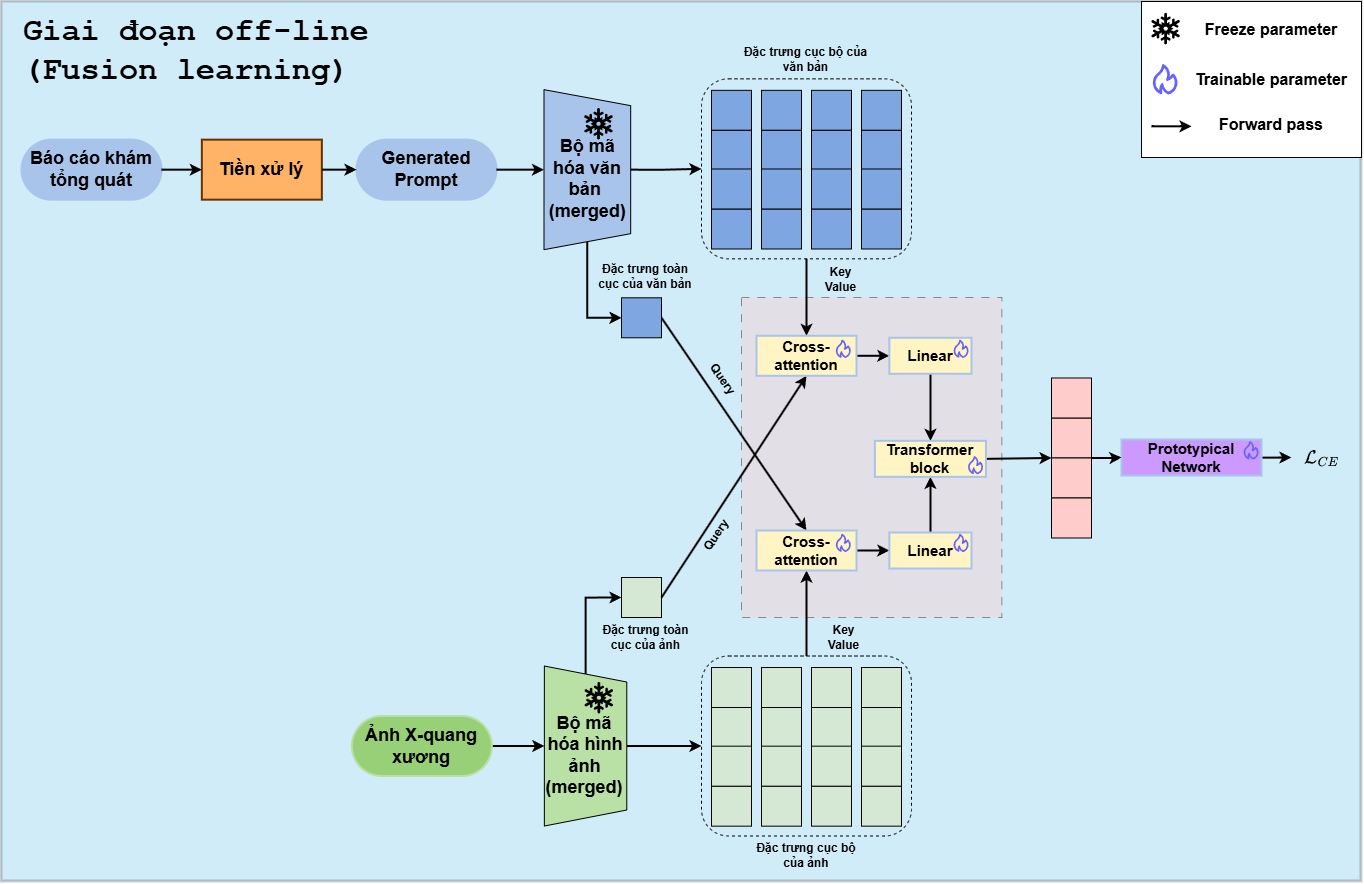
\includegraphics[width=1\linewidth]{images/fusion-learning.png}
    \caption{Sơ đồ chung của hệ thống trong công đoạn Fusion-learning.}
    \label{fig:fusion-learning}
\end{figure}
Trong công đoạn này, nhóm tối ưu khả năng khai thác và dung hợp dữ liệu bằng cách sử dụng kỹ thuật Bidirectional Cross-Attention để học các mối liên hệ giữa đặc trưng đặc trưng toàn cục của ảnh X-Quang với đặc trưng cục bộ của báo cáo khám tổng quát và ngược lại.

Để mô phỏng sát với quá trình học phân tích ảnh thực tế của bác sĩ, dữ liệu đầu vào của công đoạn này là các cặp ảnh X-quang và báo cáo khám tổng quát. Các dữ liệu này được đưa vào bộ mã hóa tương ứng để trích xuất đặc trưng. 
Kỹ thuật cross-attention được sử dụng để học các mối liên hệ giữa các đặc trưng này. Đặc trưng toàn cục của ảnh X-quang được sử dụng để tìm các đặc trưng cục bộ của báo cáo khám tổng quát có liên quan và ngược lại, 
đặc trưng toàn cục của văn bản được sử dụng để tìm các đặc trưng cục bộ của ảnh X-quang có liên quan. Sau đó, các đặc trưng có liên quan được đưa vào một khối Transformer, 
nơi chúng được kết hợp một lần nữa thông qua cơ chế attention để học sự phụ thuộc giữa các đặc trưng, tương quan ngữ nghĩa ở mức độ sâu hơn
 trước khi được đưa vào bộ phân loại cuối cùng để dự đoán nhãn bệnh lý. Sự khác biệt của dự đoán với nhãn thực tế sẽ được tính toán
  và sử dụng để cập nhật tham số của các khối Cross-Attention, Linear Projection và Transformer cũng như Classifier.

Hàm mất mát được sử dụng là Cross-Entropy Loss $\mathcal{L}_{CE}$, được định nghĩa như sau:
\begin{equation}
    \mathcal{L}_{CE} = -\frac{1}{N} \sum_{i=1}^{N} \sum_{k=1}^{K} y_{ik} \log(\hat{y}_{ik})
\end{equation}
trong đó, $N$ là kích thước mini-batch, $K$ là số lượng lớp bệnh lý, $y_{ik}$ là nhãn thực tế (one-hot encoded) của mẫu $i$ cho lớp $k$, 
và $\hat{y}_{ik}$ là xác suất dự đoán của mô hình cho lớp $k$ của mẫu $i$. Bằng cách tối ưu $\mathcal{L}_{CE}$, 
mô hình học được cách phân loại chính xác các bệnh lý dựa trên sự kết hợp của thông tin hình ảnh và văn bản, 
đồng thời cơ chế cross-attention và khối Transformer giúp mô hình học được các mối liên hệ phức tạp giữa hai nguồn dữ liệu này, 
từ đó cải thiện hiệu suất phân loại và khả năng giải thích của mô hình.

Nhóm đồng thời sử dụng phương pháp phân loại metric-based few-shot learning với một prototypical network, 
nhãn được quyết định bởi khoảng cách đến các prototype trong không gian biểu diễn chung, 
thay vì lớp phân loại truyền thống làm ràng buộc mô hình phân loại vào các nhãn đã biết, 
giúp phát hiện dữ liệu ngoài phân phối khi khoảng cách đó vượt quá ngưỡng xác định.

\begin{figure}[H]
    \centering
    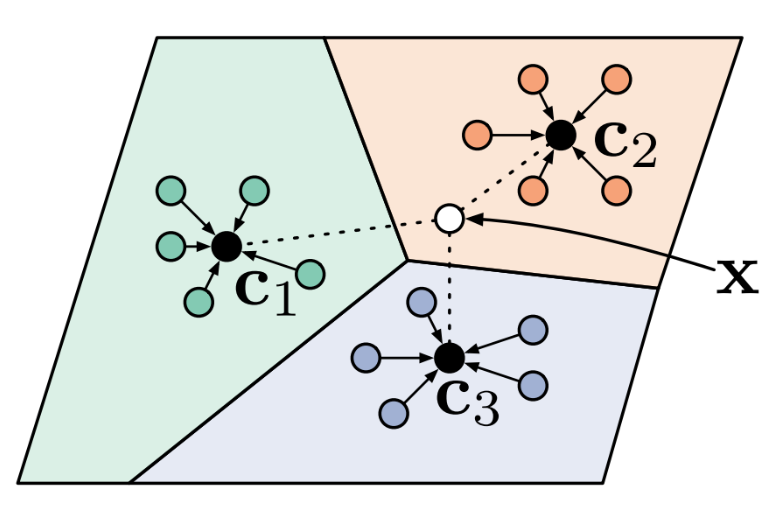
\includegraphics[width=1\linewidth]{images/prototypical_network.png}
    \caption{Sơ đồ mạng prototypical.}
    \label{fig:prototypical-network}
\end{figure}

Mỗi prototype của một lớp bệnh lý được tính bằng cách lấy trung bình của các đặc trưng của các mẫu hỗ trợ (support samples) thuộc lớp đó trong không gian biểu diễn chung.
\begin{equation}
c_k=\frac{1}{|S_k|}\sum_{(x_i,y_i)\in S_k} f(x_i)
\end{equation}

Trong đó, $c_k$ là prototype của lớp $k$, $S_k$ là tập các mẫu hỗ trợ thuộc lớp $k$, và $f(x_i)$ là đặc trưng của mẫu $x_i$ được trích xuất bởi mô hình.

% Euclidean distance giữa embedding và prototype
Khoảng cách giữa embedding của mẫu cần phân loại và prototype của lớp được tính bằng khoảng cách Euclidean:
\begin{equation}
d(z,c_k)=\|z-c_k\|^2
\end{equation}

Xác suất dự đoán của mẫu $x$ thuộc lớp $k$ được tính bằng hàm softmax trên các khoảng cách đến các prototype:
\begin{equation}
p(y=k|x)=\frac{\exp(-d(z,c_k))}{\sum_{j=1}^{K} \exp(-d(z,c_j))}
\end{equation}

Trong đó, $z$ là embedding của mẫu $x$ được trích xuất bởi mô hình. Bằng cách sử dụng phương pháp phân loại này, mô hình có thể dự đoán nhãn cho các mẫu mới dựa trên khoảng cách đến các prototype,
đồng thời có khả năng phát hiện dữ liệu ngoài phân phối khi khoảng cách đó vượt quá ngưỡng xác định.

Hàm mất mát được sử dụng để tối ưu là Cross-Entropy Loss $\mathcal{L}_{CE}$, được định nghĩa như sau:
\begin{equation}
    \mathcal{L}_{CE} = -\frac{1}{N} \sum_{i=1}^{N} \sum_{k=1}^{K} y_{ik} \log(p(y=k|x_i))
\end{equation}
trong đó, $N$ là kích thước mini-batch, $K$ là số lượng lớp bệnh lý, $y_{ik}$ là nhãn thực tế (one-hot encoded) của mẫu $i$ cho lớp $k$, và $p(y=k|x_i)$
là xác suất dự đoán của mô hình cho lớp $k$ của mẫu $i$ được tính bằng hàm softmax trên các khoảng cách đến các prototype. Bằng cách tối ưu $\mathcal{L}_{CE}$,
mô hình học được cách phân loại chính xác các bệnh lý dựa trên sự kết hợp của thông tin hình ảnh và văn bản,
đồng thời cơ chế cross-attention và khối Transformer giúp mô hình học được các mối liên hệ phức tạp giữa hai nguồn dữ liệu này,
từ đó cải thiện hiệu suất phân loại và khả năng giải thích của mô hình.

\section{Giai đoạn online}
\begin{figure}[H]
    \centering
    
\includegraphics[width=1\linewidth]{images/online.png}
    \caption{Sơ đồ chung của hệ thống trong giai đoạn online.}
    \label{fig:online}
\end{figure}

Sơ đồ của hệ thống trong giai đoạn online được trình bày trong Hình \ref{fig:online}. Gần tương ứng với công đoạn Fine-tuning, 
ảnh X-Quang cùng báo cáo tổng quát gồm lời khai của bệnh nhân và tiền sử bệnh lý sau tiền xử lí được đưa vào bộ mã hóa tương ứng để trích xuất đặc trưng.
Các đặc trưng này được đưa vào khối Cross-Attention để học các mối liên hệ tương tác giữa đặc trưng toàn cục với các đặc trưng cục bộ, 
sau đó được đưa vào khối Transformer để hợp nhất đặc trưng đa phương thức ở mức độ sâu hơn trước khi được đưa vào mạng prototypical để dự đoán nhãn bệnh lý, 
ở đây, nhãn được lựa chọn dựa trên khoảng cách đến các prototype, nếu khoảng cách đến prototype gần nhất vượt quá ngưỡng nhất định, mô hình sẽ đánh dấu là không chắc chắn.
Ngoài ra, các trọng số attention và thông tin từ tri thức y khoa được khai thác để trực quan hóa và giải thích kết quả dự đoán. 
Cụ thể, mô hình có thể tạo ra các bản đồ nhiệt trực quan hóa trên ảnh X-quang dựa trên các trọng số attention để giải thích dự đoán của mô hình.

\section{Đóng góp của phương pháp}
\begin{itemize}
    \item \textbf{Tích hợp tri thức y khoa với biểu diễn đa phương thức:} Không chỉ sử dụng kết hợp cả hai phương thức dữ liệu, 
    phương pháp đã thực hiện trích xuất các thông tin cần thiết từ văn bản y khoa theo khuôn mẫu, giúp giảm nhiễu ngôn ngữ tự nhiên, tăng tính nhất quán ngữ nghĩa; 
    đồng thời việc làm giàu tri thức qua UMLS giúp làm giàu ngữ nghĩa văn bản theo chuẩn y khoa mà không gặp vấn đề hallucination so với việc tạo ra mô tả bằng LLM.
    \item \textbf{Cơ chế Cross-Attention có hướng dẫn tri thức:} Việc sử dụng cơ chế Cross-Attention có hướng dẫn tri thức giúp mô hình tập trung vào các vùng ảnh có liên quan đến bệnh lý, 
    thay vì các vùng nền không liên quan. Điều này không chỉ cải thiện hiệu năng mà còn cung cấp khả năng giải thích thông qua việc truy vết mối liên hệ giữa khái niệm y khoa và vùng ảnh được chú ý.
    \item \textbf{Cơ chế fusion ở nhiều cấp độ:} Việc kết hợp đặc trưng toàn cục và cục bộ thông qua Cross-Attention và khối Transformer giúp mô hình khai thác tối đa dữ liệu 
    và học được các mối liên hệ phức tạp giữa hai nguồn dữ liệu, từ đó cải thiện hiệu suất phân loại và khả năng giải thích của mô hình.
    \item \textbf{Giảm nguy cơ suy giảm không gian ngữ nghĩa trong bối cảnh dữ liệu hạn chế:} 
Cơ chế cập nhật tham số bằng LoRA giúp các bộ mã hóa thích nghi với dữ liệu y khoa đích mà không làm mất mát các tri thức đã học. Điều này giúp hạn chế hiện tượng overfitting và giảm độ phức tạp tính toán.
    \item \textbf{Cơ chế phát hiện dữ liệu ngoài phân phối:} Mô hình có khả năng phát hiện dữ liệu ngoài phân phối với mạng prototypical.
\end{itemize}
